\chapter{Biological background}

\label{kap:background} % id kapitoly pre prikaz ref
\paragraph*{}
In this chapter, we explain advantages of phage therapy compared to antibiotics. We introduce biological processes happening when bacteriophage infects bacteria and the lytic properties of endolysins. We also outline chemical processes used for extraction and sequencing of bacteriophage DNA.

\section{Bacteriophages vs. Antibiotics}

\begin{figure}[h]
  \begin{center}
     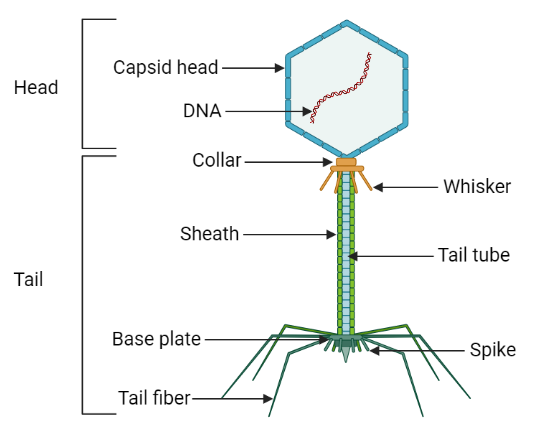
\includegraphics[width=0.5\textwidth]{images/bacteriophage.png}
     \caption{Structure of a bacteriophage.}\label{fig:phage}
  \end{center}
\end{figure} 

\paragraph*{}
Bacteriophages or phages are a type of virus which evolved specifically to be able to infect bacteria. They are composed of a molecule of nucleic acid encased in a protein structure (Figure \ref{fig:phage}). While there are thousands of varieties of phages, each phage usually infects only one type or a few types of bacteria \cite{guttman2005basic}. This characteristic is utilized in phage therapy, which uses phages as an alternative to treatment using antibiotics. 

There are two main advantages of phage therapy \cite{lin2017phage} when compared to antibiotics treatment. Antibiotics eliminate bacteria regardless of whether the bacteria is harmful, beneficial or does not affect the body. This in turn leads to damage of gut microbiota, which can create a change in bacterial metabolites, disrupt bacterial signaling and antimicrobial peptide secretion or damage regulation of function of gut immune cells \cite{zhang2019facing}. Unlike antibiotics, phage therapy targets only a specific type of bacteria allowing the body to maintain healthy microbial environment \cite{lin2017phage}. 

Another advantage is that unlike antibiotics, bacteriophages are alive and as such are subjected to evolution. Because bacteria are evolving, they are able to gain resistance to antibiotics to which they are exposed. When large variety of bacteria gain resistance to an antibiotic, the antibiotic is rendered ineffective. Similarly, when a bacteria gains resistance to multiple antibiotics, the treatment becomes even more difficult. Presently, many multiple antibiotics resistant bacteria already exist, like some strains of Staphylococus aureus or Mycobacterium tuberculosis \cite{guilfoile2007antibiotic}. As a result, it becomes necessary to develop a new antibiotic. However, this demands arduous research as well as substantial financial support. 

In contrast, when a bacteria develops resistance to a particular strain of bacteriophage, the bacteriophage as a result of its evolution develops another method of infecting that bacteria, bypassing the resistance to the virus. Since this process happens naturally, uncovering new phages capable of infecting bacteria is significantly less demanding. It also implies an inexhaustible supply of treatment for bacterial infections, which is becoming increasingly more important with bacteria gradually developing resistances to an increasing number of antibiotics.

\section{Life cycle of a phage}
\paragraph*{}
In order for the phage to infect a bacteria, its tail fibres bind to specific receptors on the surface of the bacteria. While tail fibres and receptor pairing are highly specific, different types of phages might use the same receptors on membrane \cite{guttman2005basic}. The phage then creates a puncture in the bacterial membrane. Next, the nucleic acid is expelled from the phage through its tail and injected into the bacteria. When in cytoplasm, the viral genome in some cases becomes circular and resembles plasmid. After entering the bacteria, nucleic acid enters one of two cycles: lytic or lysogenic.

\begin{figure}[h]
  \begin{center}
     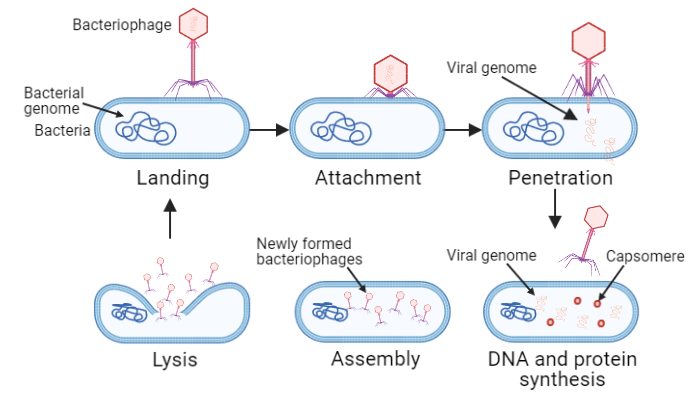
\includegraphics[width=0.5\textwidth]{images/lytic.png}
     \caption{Lytic cycle.}\label{fig:lytic}
  \end{center}
\end{figure} 

In the lytic cycle (Figure \ref{fig:lytic}), the viral nucleic acid is transcribed into messenger RNA (mRNA). If the viral genome consists of DNA, it is directly transcribed into mRNA. In case when it consists of RNA, it is first transcribed using an enzyme, reverse transcriptase, into DNA and then transcribed into mRNA. This mRNA utilizes cellular mechanisms of the host to destroy the hosts nucleic acid \cite{guttman2005basic}. After the destruction of the host nucleic acid, the viral genome is replicated and transcribed to produce proteins required for the assembly of new viruses. After enough proteins and viral genome is produced, they are assembled to create new bacteriophages. Next, the phage produces enzyme, endolysin, which causes the lysis of the cellular membrane. By destroying the membrane, newly formed bacteriophages are released, ending the lytic cycle.

\begin{figure}[h]
  \begin{center}
     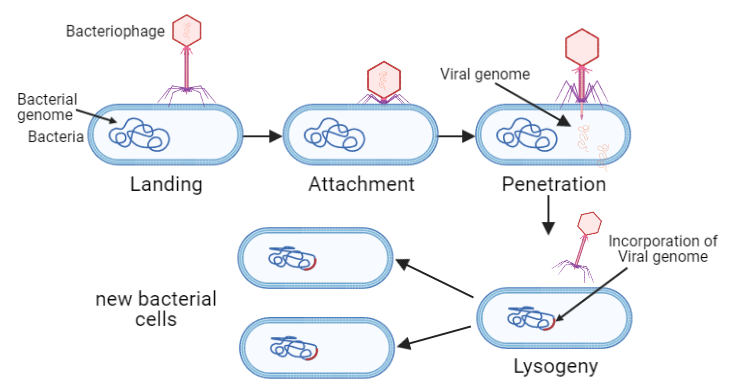
\includegraphics[width=0.5\textwidth]{images/lysogenic.png}
     \caption{Lysogenic cycle.}\label{fig:lysogenic}
  \end{center}
\end{figure} 

The lysogenic cycle (Figure \ref{fig:lysogenic}) differs from the lytic cycle by not immediately destroying the nucleic acid of the bacteria. Instead, it integrates its nucleic acid into the host genome, creating prophage. This is accomplished either by site-specific recombination or by random transposition \cite{guttman2005basic}. After integrating into the host genome, the prophage remains in a dormant state. The cellular mechanism of the bacteria remains unaffected by the prophage, so the bacteria continues its regular functions without alteration. During cell division, the prophage replicates with the host chromosomes resulting in the new bacterial cells already being infected by the phage. This process of replication is repeated until the conditions of the environment deteriorate. The deterioration can be induced by physical factors like UV radiation, low nutrient concentration or chemical factors. When the conditions deteriorate, the prophage might switch from lysogenic to the lytic cycle. 

The lysogenic cycle of the phage has the advantage of increasing the amount of bacteriophages created from a single specimen. Since the phage is replicated during cell division along with the host cell, the number of proteins required to infect the same number of hosts is halved with each division, meaning the phage utilizing lysogenic cycle can reproduce in worse conditions than a phage only utilizing the lytic cycle.


\section{Endolysins}
\paragraph*{}
Because the purpose of phage therapy is the treatment of bacterial infection, the part of bacteriophages life cycle of most interest is the production of endolysin. Endolysins, alternatively termed phage lysins, are peptidoglycan hydrolases used by bacteriophages to enzymatically degrade the cellular membrane of the host bacteria, resulting in osmotic imbalance leading to rapid lysis of the membrane \cite{schmelcher2012bacteriophage}. The structure of lysins is in big part affected by whether the targeted bacteria is Gram-positive or Gram-negative, as the cellular membrane of these groups have different structure. 

Endolysins of bacteriophages targeting Gram-positive bacteria have evolved in a way, where catalytic activity and substrate recognition are separated into two distinct varieties of functional domains, enzymatically active domains and cell wall binding domains \cite{schmelcher2012bacteriophage}. Enzymatically active domains impart the catalytic mechanism of lysin, the mechanism for cleaving of specific bonds in a cellular membrane of bacteria. The cell wall binding domain is responsible for targeting the lysin to its substrate and keeping it bound to parts of cell wall after cell lysis, reducing the probability of lysis of surrounding cells not yet infected by the phage.

On the contrary, endolysins of phages targeting Gram-negative bacteria have a tendency to be small single-domain globular proteins without a specific domain for binding to the cell wall \cite{schmelcher2012bacteriophage}. Unlike endolysins from Gram-positive background, damage to surrounding bacteria in case of Gram-negative bacteria is prevented by its characteristic outer membrane, which protects the cell wall from the outside environment. Lysin is encased in the outer membrane, resulting in prevention of damage to other bacteria. It is surmised, that these endolysins fulfill their catalytic role more effectively as opposed to endolysins for Gram-positive bacteria \cite{schmelcher2012bacteriophage}, which are bound to one site on the membrane and as such reduced effectivity.

To further increase the diversity of possible endolysin architectures, the structure of endolysins from Gram-positive background can have more than two domains. Most prominent structures include two N-terminal enzymatically active domains and one C-terminal cell wall binding domain, central cell wall binding domains separating two terminal enzymatically active domains, among others \cite{schmelcher2012bacteriophage}. Almost all currently described Gram-positive endolysins are encoded by single gene, simplifying their localization in the phage genome.

Enzymatically active domains encompass the ability of an endolysin to catalyze a breakdown of the cell membrane. Based on the bond of the cell membrane an endolysin attacks, endolysins can be classified into five different groups: N-acetyl-\textbeta-D-muramidases (lysozymes) and lytic transglycosylases that cleave one of the glycosidic bonds of a sugar strand, N-acetyl-\textbeta-D-glucosaminidases cutting another glycosidic bond in the sugar strand, N-acetylmuramoyl-L-alanine amidases hydrolysing amide bond between sugar and peptide parts and endopeptidases cleaving the peptides making up interconnecting stem portion of the membrane \cite{schmelcher2012bacteriophage}. Any of these methods lead to destabilization and breakdown of the cell membrane.

Cell wall binding domains allow an endolysin to recognise and bind (not using covalent bond) to ligands within cell membrane or other molecules associated with the cell wall. This significantly reduces range of activity for the enzymatically active domains. The spectrum of the cell wall binding domains can range from encompassing an entire genus of bacteria (lysostaphin domain targeting SH3b-like cell wall common to staphylococcal strains), making it generally broader than the host range of the particular phage, to the specificity of a single strain (endolysins of Listeria phage binding to groups of Listeria containing very specific ligands) \cite{schmelcher2012bacteriophage}.

\section{Data preparation}
\paragraph*{}
To gain usable information about bacteriophages, it is necessary to extract their DNA and be able to analyse it. As a result of the phage DNA being relatively small, the phage needs to be replicated in order to provide a viable sample. The DNA then needs to be extracted from the phage. Once the phage DNA is extracted, it can be sequenced to provide data for bioinformatic analysis. 

\subsection{Propagation and extraction}
\paragraph*{}
The propagation and extraction of phage DNA are dependent on the species of phage in question \cite{kleiner2015evaluation}. In general, however, the process is carried out by following similar steps. Since phages do not have their own replication apparatus, in order to acquire sufficient amount of DNA for sequencing, it is necessary to utilize the replication apparatus of bacteria. For this purpose, bacterial hosts are first grown independently in advantageous environment.

Once the hosts are sufficiently grown, a solution containing phages is mixed in with the host culture. The resulting culture is then incubated in order to facilitate phage replication. In the process, the lysis of the host is achieved, releasing the replicated phages into the environment. After a period of time, the culture is transferred to a centrifuge and spun. The bacterial pellet is settled at the bottom of the substrate is discarded while the remaining supernatant is kept. The resulting substrate is then treated with RNase and DNase. After, a solution of NaCl and PEG (poly(ethylene glycol)) is added to the culture and incubated. As a result, the phage particles then precipitate. 

Resulting substrate is then centrifuged, creating a phage pellet from the precipitated particles. The pellet is extracted from the substrate and resuspended in a buffer. To remove phage protein capsid, phenol is added and the substrate is incubated. After the protein dissolves, the aqueous layer is removed. Ethanol is then added to the DNA and the substrate is centrifuged. Finally, extracted DNA is concentrated.

\subsection{Sequencing}
\paragraph*{}
After the extraction of phage DNA is completed, the DNA needs to be sequenced in order to be analysed by our tool. There are many ways to sequence DNA. Since our tool is specialized to work with reads from Illumina sequencers, the process of sequencing described is focused on Illumina MiSeq \cite{ravi2018miseq}.

\begin{figure}[h]
  \begin{center}
     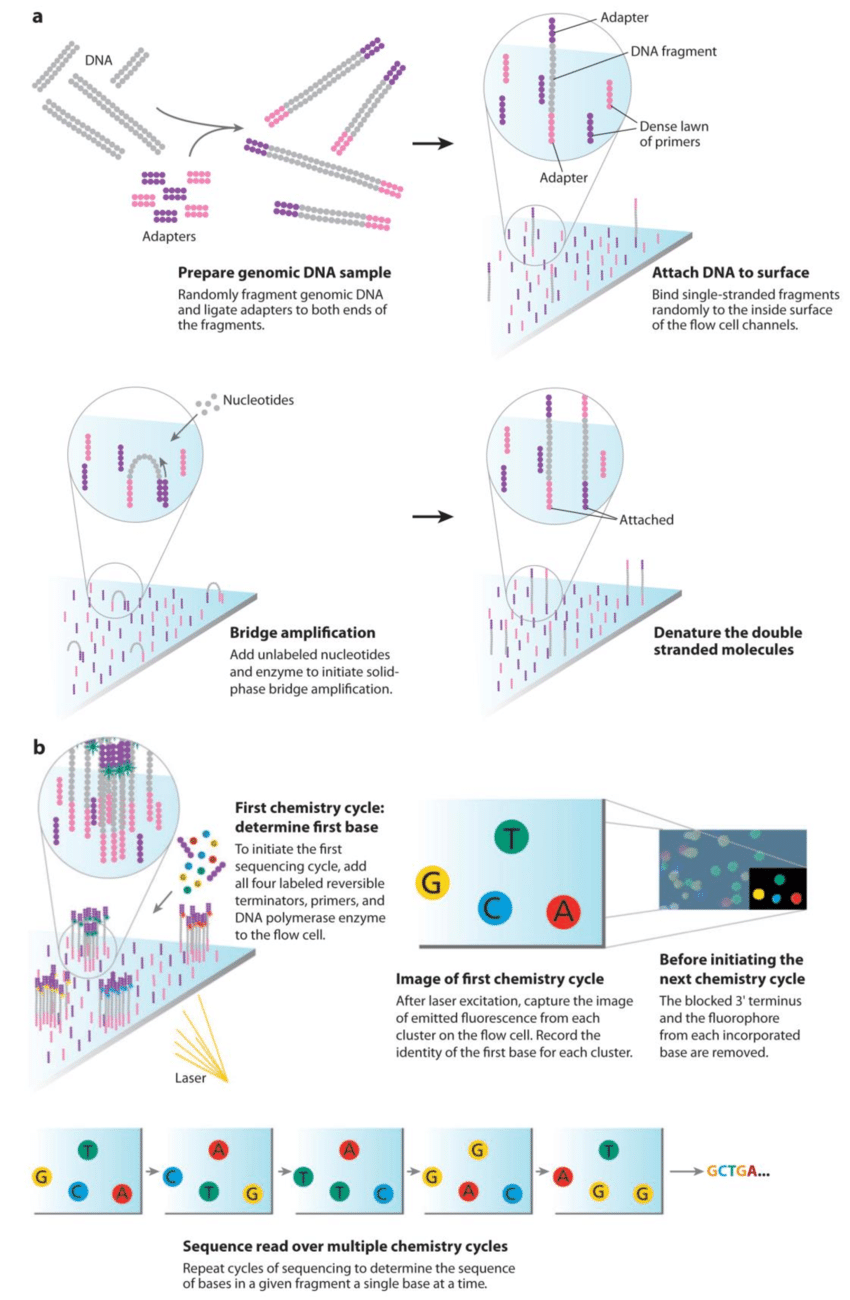
\includegraphics[width=0.5\textwidth]{images/sequencing.png}
     \caption{Library preparation (a) and sequencing (b) using Illumina Miseq\cite{phdthesis}.}\label{fig:sequencing}
  \end{center}
\end{figure} 

Before starting the sequencing, the sequencer requires a DNA library (Figure \ref{fig:sequencing}a). To create a DNA library, DNA is first fragmented into small parts (500-1000 bp). After addition of special barcoding sequences to the fragments, short oligonucleotides (adaptors) are bound to the fragments. The adaptors are complementary to primer sequences on a glass disc. The fragment is attached to the glass disc by a primer on one end, while the other is held close to another primer using its adaptor. After the attachment to the glass disc, a new strand of DNA complementary to the attached strand is synthesized. This new strand is attached to the primer the first strand is held close to by its adaptor. After the synthesis, the two strands separate, and the bond between the adaptor and the primer is released. This form of replication is repeated many times, creating thousands of copies of the fragment in close proximity forming a cluster. This happens on the glass disc for every fragment of DNA, creating a DNA library.

With the library created, the sequencing can proceed (Figure \ref{fig:sequencing}b). During sequencing, a substrate called "mastermix" is used. Mastermix contains primers, DNA-polymerase and 4 different types of marked fluorescent nucleotides with a sequence inhibiting polymerization (terminators) on its 3' -end. The nucleotides are bound to the fragments of DNA based on complementarity. Next, the excess mastermix is removed from the disc. The sequencer then measures fluorescence of the bound nucleotides to determine their identity. After the measurement, the terminators split from the sequence allowing another nucleotide to connect. This process is cyclically repeated until the entire library is read. The result is a set of sequences of DNA with adaptor sequences. These sequences are then processed by bioinformatic pipelines.
